% !TEX encoding = UTF-8 Unicode
\documentclass[titlepage]{report}
%\documentclass[fontsize=12pt]{article}

\usepackage[utf8]{inputenc}
\usepackage[T1]{fontenc}
\usepackage{illcmolthesis}
\usepackage[a4paper, margin=1.08in]{geometry}
\usepackage{amsmath}
\usepackage{amsfonts}
\usepackage{amssymb}
\usepackage[mathscr]{eucal}
\usepackage{enumitem}
\usepackage{mathtools}
\usepackage{IEEEtrantools}
\usepackage[backend=bibtex]{biblatex}
\usepackage{indentfirst}
\usepackage{physics}
\usepackage{bm}
\usepackage{mathtools}
\usepackage{etoolbox}
\usepackage{xifthen}
\usepackage{ulem}
\usepackage{titlesec}
\usepackage{hyperref}
\usepackage{float}
\usepackage[ruled, linesnumbered, noalgohanging]{algorithm2e}
\usepackage{graphicx}
\usepackage{subcaption}
\usepackage{booktabs}

\addbibresource{references.bib}

\newcounter{theorem}
\newcounter{lemma}

\newcommand\where[1][\big]{\:#1\vert\:}
\newcommand{\otoprule}{\midrule[\heavyrulewidth]}
\DeclareMathOperator*{\argmin}{arg\,min}
\DeclareMathOperator*{\argmax}{arg\,max}
\DeclareMathOperator{\softmax}{softmax}
\DeclareMathOperator{\score}{score}
\DeclareMathOperator{\aln}{align}
\DeclareMathOperator{\relu}{ReLU}
\DeclareMathOperator{\CTM}{CTM}
\DeclareMathOperator{\BDM}{BDM}

\restylefloat{table}

\makeatletter
\newcommand{\RemoveAlgoNumber}{\renewcommand{\fnum@algocf}{\AlCapSty{\AlCapFnt\algorithmcfname}}}
\newcommand{\RevertAlgoNumber}{\algocf@resetfnum}
\makeatother

%\setul{5pt}{.4pt}

\newenvironment{def*}[1][]
	{%
	\par\addvspace{9pt}%
	\noindent%
	\uline{\textbf{Definition%
	\ifthenelse{\isempty{#1}}%
		{}%
		{ (#1)}%
	}}%
	\hspace{5pt}%
	\ignorespaces%
	}
	{%
	\par\addvspace{9pt}%
	}

\newenvironment{theorem}[1][]
	{%
	\stepcounter{theorem}%
	\par\addvspace{9pt}%
	\noindent%
	\uline{\textbf{Theorem \thetheorem%
	\ifthenelse{\isempty{#1}}%
		{}%
		{ (#1)}%
	}}%
	\hspace{5pt}%
	\ignorespaces%
	}
	{%
	\par\addvspace{9pt}%
	}

\newenvironment{proof}[1][]
	{%
	\par\addvspace{9pt}%
	\noindent%
	\uline{\textbf{Proof%
	\ifthenelse{\isempty{#1}}%
		{}%
		{ (#1)}%
	}}%
	\hspace{5pt}%
	\ignorespaces%
	}
	{%
	\hfill%
	$\square$%
	\par\addvspace{9pt}%
	}

\newenvironment{lemma}[1][]
	{%
	\stepcounter{theorem}%
	\par\addvspace{9pt}%
	\noindent%
	\uline{\textbf{Lemma \thetheorem%
	\ifthenelse{\isempty{#1}}%
		{}%
		{ (#1)}%
	}}%
	\hspace{5pt}%
	\ignorespaces%
	}
	{%
	\par\addvspace{9pt}%
	}

\newenvironment{corollary}[1][]
	{%
	\stepcounter{theorem}%
	\par\addvspace{9pt}%
	\noindent%
	\uline{\textbf{Corollary \thetheorem%
	\ifthenelse{\isempty{#1}}%
		{}%
		{ (#1)}%
	}}%
	\hspace{5pt}%
	\ignorespaces%
	}
	{%
	\par\addvspace{9pt}%
	}

\newenvironment{corollary*}[1][]
	{
	\par\addvspace{9pt}%
	\noindent%
	\uline{\textbf{Corollary%
	\ifthenelse{\isempty{#1}}%
		{}%
		{ (#1)}%
	}}%
	\hspace{5pt}%
	\ignorespaces%
	}
	{%
	\par\addvspace{9pt}%
	}

\newenvironment{example*}[1][]
	{
	\par\addvspace{9pt}%
	\noindent%
	\uline{\textbf{Example%
	\ifthenelse{\isempty{#1}}%
		{}%
		{ (#1)}%
	}}%
	\hspace{5pt}%
	\ignorespaces%
	}
	{%
	\par\addvspace{9pt}%
	}

\titlespacing{\section}{0pt}{24pt}{18pt}

\hypersetup{
	colorlinks = true,
	urlcolor = blue
}

\title{THESIS TITLE}
\author{Krsto Proroković}
\birthdate{March 12, 1993}
\birthplace{Kotor, Montenegro}
\defensedate{Date of the defense goes here}
\supervisor{Dr Germán Kruszewski}
\supervisor{Dr Elia Bruni}
\committeemember{Committee goes here}

\setlength{\parindent}{12pt}

\begin{document}

\maketitle
\RemoveAlgoNumber

\begin{abstract}
Abstract goes here
\end{abstract}

\chapter*{Acknowledgents}

\tableofcontents

\chapter{Introduction}

\chapter{Related Work}

Learning to decide a formal language can be seen as an example of learning an algorithm from input/output examples. There are several approaches to this problem. One would be to induce a discrete program from finite set of instructions. Inductive logic programming \cite{muggleton1991inductive} requires domain specific knowledge about the programming languages and hand-crafted heuristics to speed up the underlying combinatorial search. Levin \cite{levin1973universal} devised an asymptotically optimal method for inverting functions on given output, albeit with a large constant factor. Hutter \cite{hutter2002fastest} reduced the constant factor to less than 5 at the expense of introducing a large additive constant. These methods are not incremental and do not make use of machine learning. Schmidhuber \cite{schmidhuber2004optimal} extended the principles of Levin's and Hutter's method and developed an asymptotically optimal, incremental method that learns from experience. However, the constants involved in the method are still large which limits its practical use.

The approach that we will take over here is based on training differentiable neural networks. To the best of our knowledge no one used neural networks for deciding a whole class of formal languages, rather a single language from positive and negative examples. Mozer and Das \cite{mozer1993connectionist} used neural networks with external stack memory to parse simple context-free languages such as $a^n b^n$ and parenthesis balancing from both positive and negative examples. Wiles and Elman \cite{wiles1995learning} used neural networks to learn sequences of the form $a^n b^n$ and generalise on a limited range of $n$. Joulin and Mikolov \cite{joulin2015inferring} used recurrent neural networks augmented with a trainable memory to predict the next symbol of the element of context-free language. Lastly, Zaremba and Sutskever \cite{zaremba2014learning} used recurrent neural networks for learning to execute simple Python programs.

\chapter{Background}

In this chapter we ...

\section{Locally k-testable languages}

Fix an alphabet $\mathcal{A} = \{ a_1, a_2, \ldots, a_n \}$. An $SL_k$ definition is just a set of blocks of $k$ adjacent symbols (called $k$-factors) drawn from the alphabet. A string satisfies the description if and only if every $k$-factor that occurs in the string is licensed by the definition. We can see $k$-factors as atomic properties of strings: a string satisfies a $k$-factor if and only if that factor occurs somewhere in the string. Then, we can build descriptions as propositional formulas over these atoms. We will call these formulas $k$-expressions. A $k$-expression defines the set of all strings that satisfy it. A language that is defined in this way is called a locally $k$-testable ($LT_k$) language.
\par
A scanner for an $LT_k$ language contains a table in which it records, for every k-factor over the alphabet, whether or not that $k$-factor has occurred somewhere in the string. It then feeds this information into a Boolean network which implements some $k$-expression. When the end of the string is reached, the automaton accepts or rejects the string depending on the output of the network.

\begin{center}
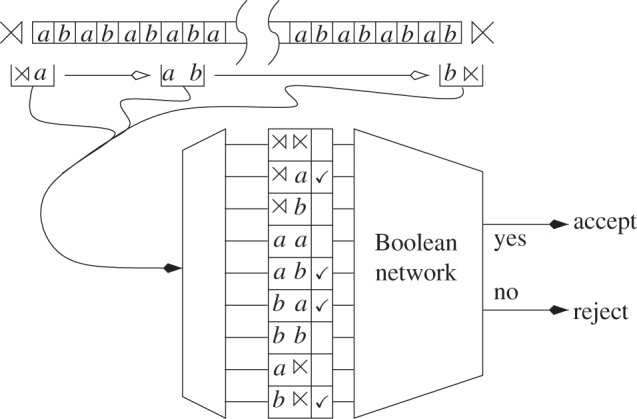
\includegraphics[width=80mm]{figures/locally_k-testable.jpg}
\end{center}

\section{Recurrent Neural Networks}

Recurrent neural networks (RNNs) \cite{rumelhart1985learning} are parametric models of computation for processing sequences loosely inspired by biological neural networks. They found applications in handwriting recognition [reference], speech recognition [reference], machine translation [reference], etc. In this section we provide an introduction to RNNs and ... For a more detailed treatment we point the reader to \cite{graves2012supervised}.

\subsection{Vanilla Recurrent Neural Networks}

We start with a simple vanilla RNN model. A vanilla RNN is given with the following parameters:

\begin{itemize}[itemsep = -2pt]
\item Input to hidden connection weights $\mathbf{W}^{\mathbf{x}} \in \mathbb{R}^{d_h \times d_x}$
\item Hidden to hidden connection weights $\mathbf{W}^{\mathbf{h}} \in \mathbb{R}^{d_h \times d_h}$
\item Bias term $\mathbf{b}^{\mathbf{h}} \in \mathbb{R}^{d_h}$
\item Activation function $\phi: \mathbb{R} \to \mathbb{R}$
\item Hidden to output connection weights $W_y \in \mathbb{R}^{d_y \times d_h}$
\item Bias term $\mathbf{b}^{\mathbf{y}} \in \mathbb{R}^{d_y}$
\item Initial hidden state $h^{(0)} \in \mathbb{R}^{d_h}$ (usually set to zero vector)
\end{itemize}

\noindent
Connection weights model the strength of synapses and activation function models neuronal firing \cite{llinas2008neuron}. Most commonly used activation functions are sigmoid $\sigma(x) = 1 / (1 + \exp(-x))$, hyperbolic tangent $\tanh(x) = (\exp(x) - \exp(-x)) / (\exp(x) + \exp(-x))$ and rectified linear unit $\relu(x) = \max \{ 0, x \}$.

%\begin{IEEEeqnarray*}{rcl}
%\text{sigmoid} \: \sigma(z) &= \frac{1}{1 + \exp(-z)} & \includegraphics[width=60mm]{sigma} \\
%\text{sigmoid} \: \sigma(z) &= \frac{1}{1 + \exp(-z)} & \includegraphics[width=60mm]{sigma}
%\end{IEEEeqnarray*}

\begin{center}
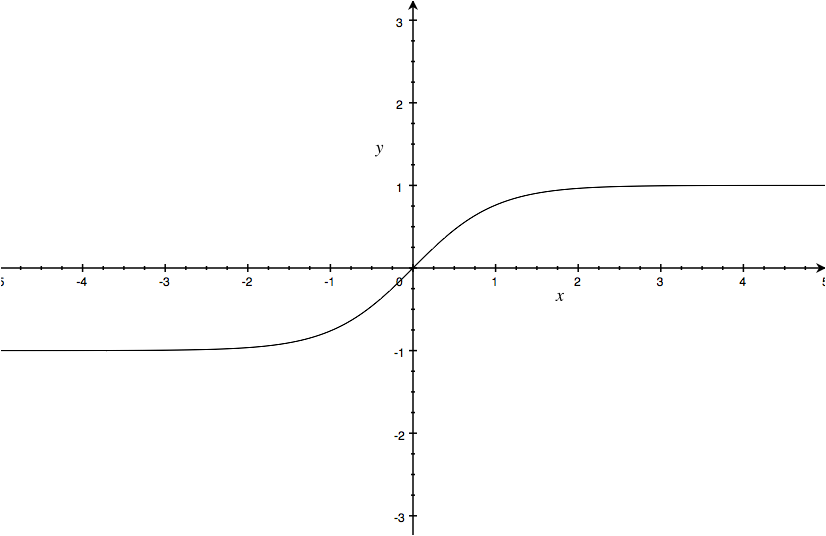
\includegraphics[width=60mm]{figures/tanh} \\
\includegraphics[width=60mm]{figures/sigma} \\
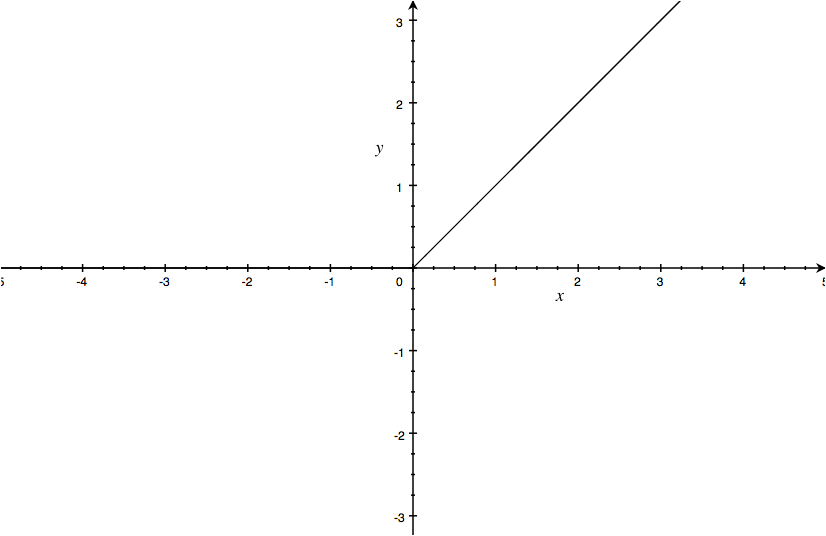
\includegraphics[width=60mm]{figures/relu}
\end{center}

\noindent
The computation is performed in the following way: for $t = 1, 2, \ldots, T$
\begin{align*}
\mathbf{h}^{(t)} &= \boldsymbol{\phi} \left( \mathbf{W}^{\mathbf{h}} \, \mathbf{h}^{(t - 1)} + \mathbf{W}^{\mathbf{x}} \, \mathbf{x}^{(t)} + \mathbf{b}^{\mathbf{h}} \right) \\
\mathbf{y}^{(t)} &= \softmax \left( \mathbf{W}^{\mathbf{y}} \, \mathbf{h}^{(t - 1)} + \mathbf{b}^{\mathbf{y}} \right)
\end{align*}

\noindent
where $\boldsymbol{\phi}(v)_i = \phi(v_i)$ and $\softmax(v)_i = \exp(v_i) / \sum_j \exp(v_j)$. 

\begin{center}
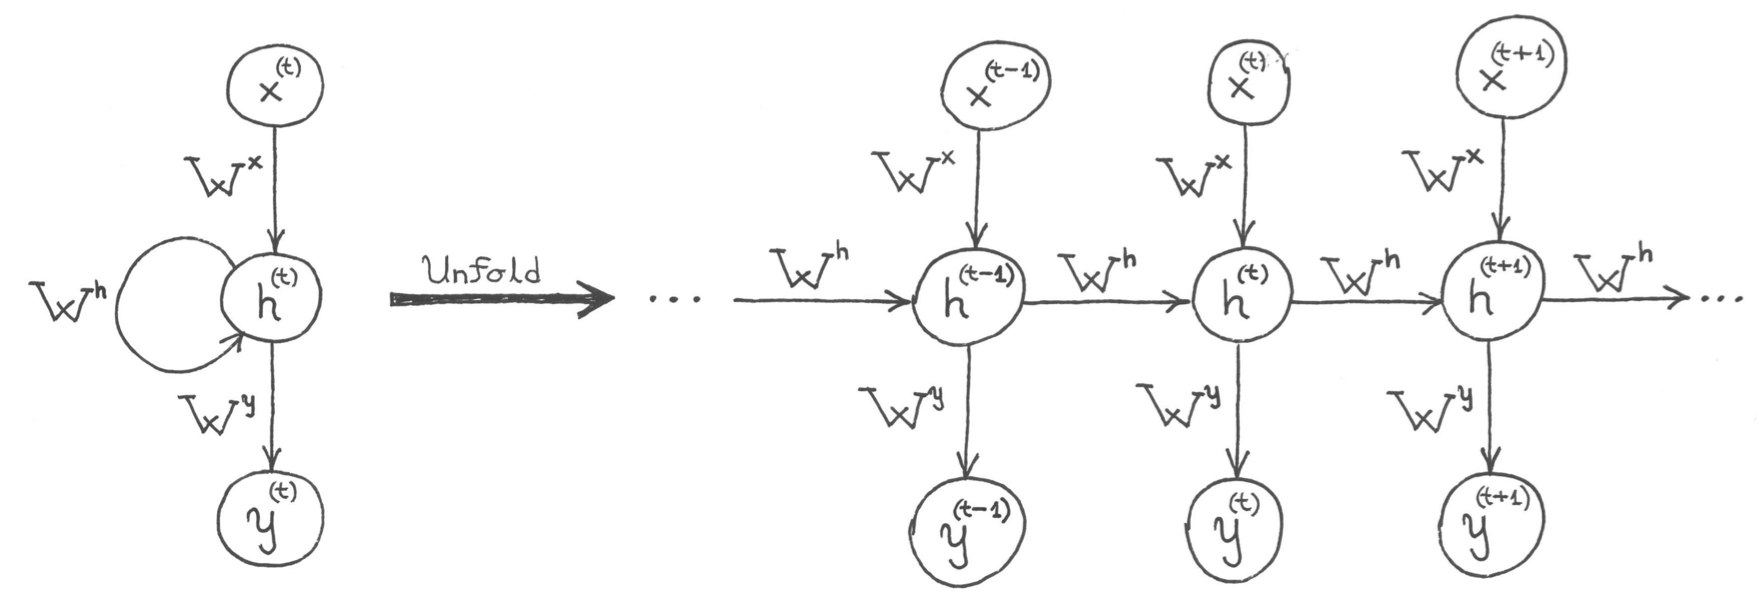
\includegraphics[width=150mm]{figures/rnn}
\end{center}

\noindent
Note that components of $y^{(t)}$ sum up to one, so we can interpret it as a probability distribution. Here we will be mostly interested in sequence classification, i.e. we will only care about $y^{(T)}$.

\begin{example*}
Consider a vanilla RNN given with the following parameters
\begin{equation*}
W_x = \begin{bmatrix} 3 & -1 & 0 \\ 0 & 0 & 2 \end{bmatrix} \quad
W_h = \begin{bmatrix} 1 & 0 \\ 0 & 1 \end{bmatrix} \quad
b_h = \begin{bmatrix} 0 \\ 0 \end{bmatrix} \quad
W_y = \begin{bmatrix} 1 & 0 \\ 0 & 1 \end{bmatrix} \quad
b_y = \begin{bmatrix} 0 \\ 0 \end{bmatrix}
\end{equation*}
\end{example*}

\noindent
and $\phi(z) = z$. It is easy to see that $y_1^{(T)} < y_2^{(T)}$ if and only if $\sum_t ( 3 x_1^{(t)} - x_2^{(t)} ) < \sum_t 2 x_3^{(t)}$. Note that in this case $h^{(t)}$ accumulates the results of the computation on the input encountered so far. \\
%$h^{(t)} = \sum_t$ ... \\

While the previous example displays a rather simple function, vanilla RNNs are universal in the sense that any function computable by a Turing machine can be computed by such a network [reference Siegelmann and Sontag].

We can also stack several RNN cells in order to exploit compositionality and obtain more powerful RNNs. Such RNNs are called multilayer or deep RNNs. The computation performed by an $L$ layer vanilla RNN is given with
\begin{align*}
\mathbf{h}_1^{(t)} &= \boldsymbol{\phi} \left( \mathbf{W}^{\mathbf{h}_1 \mathbf{h}_1} \, \mathbf{h}_1^{(t - 1)} + \mathbf{W}^{\mathbf{x} \mathbf{h}_1} \, \mathbf{x}^{(t)} + \mathbf{b}^{\mathbf{h}_1} \right) \\
\mathbf{h}_2^{(t)} &= \boldsymbol{\phi} \left( \mathbf{W}^{\mathbf{h}_2 \mathbf{h}_2} \, \mathbf{h}_2^{(t - 1)} + \mathbf{W}^{\mathbf{h}_1 \mathbf{h}_2} \, \mathbf{h}_1^{(t)} + \mathbf{b}^{\mathbf{h}_2} \right) \\
& \enspace \vdots \\
\mathbf{h}_L^{(t)} &= \boldsymbol{\phi} \left( \mathbf{W}^{\mathbf{h}_L \mathbf{h}_L} \, \mathbf{h}_L^{(t - 1)} + \mathbf{W}^{\mathbf{h}_{L-1} \mathbf{h}_L} \, \mathbf{x}^{(t)} + \mathbf{b}^{\mathbf{h}_L} \right) \\
\mathbf{y}^{(t)} &= \softmax \left( \mathbf{W}^{\mathbf{y}} \, \mathbf{h}_L^{(t - 1)} + \mathbf{b}^{\mathbf{y}} \right)
\end{align*}

\begin{center}
%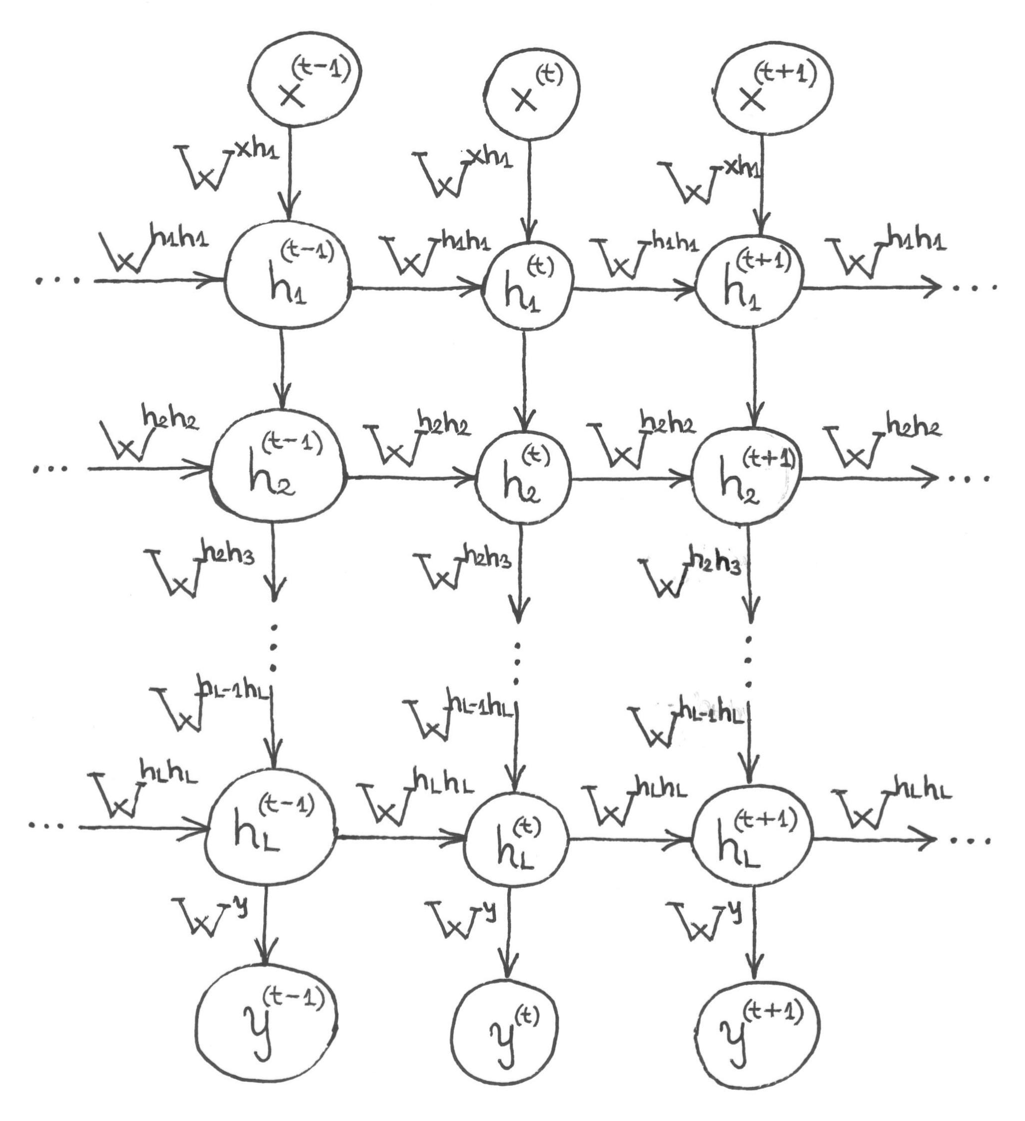
\includegraphics[width=120mm]{deep_rnn}
\end{center}

Observe that we will need $L$ initial states $\mathbf{h}_1^{(0)}, \mathbf{h}_2^{(0)}, \ldots, \mathbf{h}_L^{(0)}$.

\subsection{Backpropagation Through Time and Vanishing Gradient}

In practice we need to estimate the parameters of RNN from the data. The way this is done is by minimising the average of a certain loss function which measures how far are the outputs of the network from actual data. Suppose that we are given a dataset $\mathcal{D} = \{ (\mathbf{x}_1, \mathbf{y}_1), (\mathbf{x}_2, \mathbf{y}_2), \ldots, (\mathbf{x}_n, \mathbf{y}_n) \}$. The quantity that we are supposed to minimise is

\begin{equation*}
\mathcal{L}(\theta) = \frac{1}{n} \sum_{i = 1}^n \ell(\mathbf{y}_i, \mathbf{\hat{y}}_i)
\end{equation*}
where $\theta$ are parameters of the network and $\mathbf{\hat{y}}_i$ is the output of the network on input $\mathbf{x}_i$. The loss function that we will use here is the cross entropy loss given with
\begin{equation*}
\ell(\mathbf{y}, \mathbf{\hat{y}}) = - \sum_i y_i \log \hat{y}_i \: .
\end{equation*}

\noindent
In order to minimise the loss function we need to calculate its gradient with respect to the parameters of the network. This is achieved by Backpropagation Through Time algorithm \cite{werbos1990backpropagation}.

Unfortunately, for vanilla RNNs this does not solve the optimisation problem. The reason is that is that the gradient of the loss function may vanish or explode over many time steps. This problem has been studied independently by separate researchers [Hochreiter][Bengio]. For survey see [paper by Pascanu and Bengio].

The problem of exploding gradient can be solved by gradient clipping: if the norm of the gradient exceeds a certain threshold, then normalise it and multiply it by that threshold.
However, the vanishing gradient remains a problem for vanilla RNNs which makes their optimisation difficult in practice.

\subsection{Long-Short Term Memory Networks}

One way to deal with vanishing gradient is to use gated RNNs whose connection weights may change at each time step. Multiplicative gates allow RNNs to control the way information is stored and retrieved. Thus, they are able to create paths through time that have derivatives that neither vanish nor explode. Gates in RNNs can be seen as differentiable version of logic gates in digital circuits.
\par
Long short term memory (LSTM) networks \cite{hochreiter1997long} 
%... Apart from hidden state $h^{(t)}$ LSTM uses 
use additional memory cell $c^{(t)}$ apart from $h^{(t)}$. Here we will be using standard LSTM architecture introduced in \cite{gers1999learning} which uses four gates: forget gate $f^{(t)}$, input gate $i^{(t)}$, output gate $o^{(t)}$ and input modulation gate $g^{(t)}$. Its cell is described by the following set of equations
\begin{IEEEeqnarray*}{cl}
\begin{bmatrix} f^{(t)} \\ i^{(t)} \\ o^{(t)} \\ g^{(t)} \end{bmatrix} &= W_x x^{(t)} + W_h h^{(t)} + b \\
c^{(t)} &= \sigma(f^{(t)}) \odot c^{(t-1)} + \sigma(i^{(t)}) \odot \tanh(g^{(t)}) \\
h^{(t)} &= \sigma(o^{(t)}) \odot \tanh(c^{(t)})
\end{IEEEeqnarray*}

\noindent
where $\odot$ is component-wise or Hadamard product.

\begin{center}
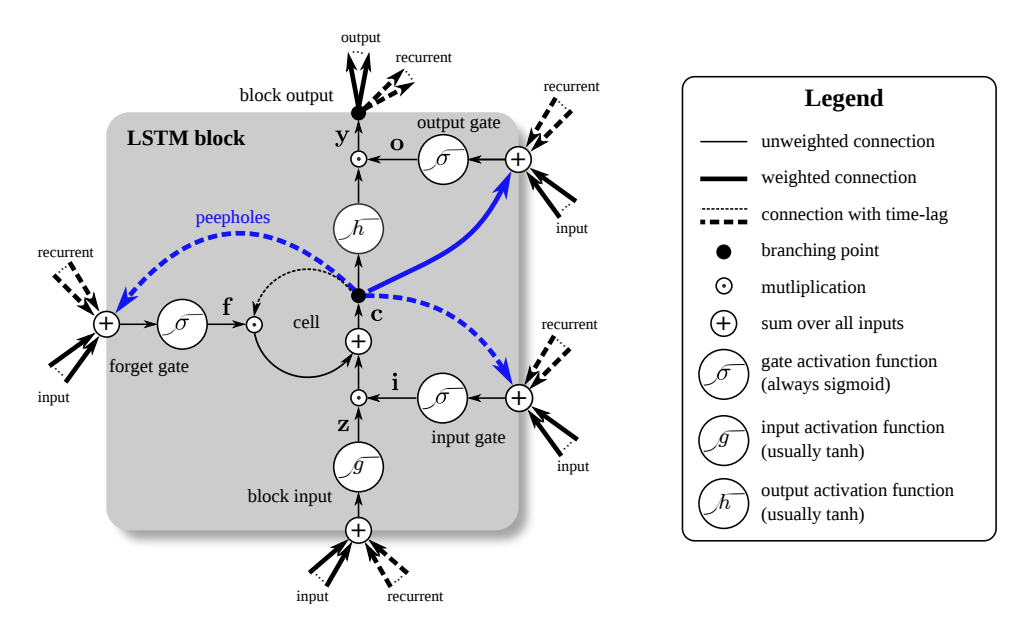
\includegraphics[width=120mm]{figures/lstm}
\end{center}

Just like vanilla RNN cells, LSTM cells can be stacked in order to obtain more powerful multilayer LSTM networks.

LSTM networks have been successfully applied in many contexts such as handwriting recognition [reference] and generation, language modeling [reference], machine translation [reference], image captioning [reference], parsing [reference], etc.

\subsection{Gated Recurrent Units}

Another gated recurrent architecture frequently used in practice are Gated Recurrent Units (GRU) \cite{cho2014learning}. Unlike LSTM, GRU gets rid of memory cell $c^{(t)}$ by combining input and forget gates into a single one. The GRU cell is described by the following set of equations
\begin{IEEEeqnarray*}{cl}
r^{(t)} &= \sigma(W_{xr} x_t + W_{hr} h^{(t-1)} + b_r) \\
z^{(t)} &= \sigma(W_{xr} x_t + W_{hz} h^{(t-1)} + b_z) \\
n^{(t)} &= \tanh(W_{xn} x_t + r_t (W_{hn} h^{(t-1)} + b_n)) \\
h^{(t)} &= (1 - z_t) n_t + z_t h_{t-1}
\end{IEEEeqnarray*}

\begin{center}
GRU figure goes here.
\end{center}

Again, GRU cells can be stacked, yielding multilayer GRU networks.

\subsection{One-hot and Dense Encodings}

Note that RNNs work exclusively with numerical data, i.e. real numbers. Suppose that we are given an alphabet $\mathcal{A} = \{ a_1, a_2, \ldots a_k \}$. One way to encode it would be to map each $a_i$ to $i$. However, this is not a good encoding as the network would need to learn that there is no ordering between alphabet elements. A better way to encode the alphabet that avoids this problem is to assign a one-hot vector to every element of the alphabet, i.e.
\begin{equation*}
a_1 \mapsto \begin{bmatrix} 1 \\ 0 \\ \vdots \\ 0 \end{bmatrix} \quad
a_2 \mapsto \begin{bmatrix} 0 \\ 1 \\ \vdots \\ 0 \end{bmatrix} \quad
\ldots \quad
a_k \mapsto \begin{bmatrix} 0 \\ 0 \\ \vdots \\ 1 \end{bmatrix}
\end{equation*}

One problem with this encoding is that $k$ may be huge while one-hot vectors remain sparse. For example, in natural language processing $k$ would be the number of words which is usually several tens of thousands. This problem is solved by using embedding layer which learns to map alphabet elements to dense, low-dimensional encodings.

\subsection{Encoder-Decoder Sequence to Sequence Models}

\subsection{Attention Mechanism}

When processing the input, RNNs store all the memory in the hidden state. However, it may be hard to compress potentially long input in a single context vector.
This could definitely be an issue if the hidden state is passed as input to another network which is common in sequence to sequence learning. For example, the family of models used for machine translation has one RNN called encoder to process the input in one language and pass it to the other RNN called decoder which is supposed to output a sequence in a different language.

Attention mechanism allows us to obtain a distribution on part of the input provided so far and focus on certain parts of it in a way we humans do. The attentional hidden state is defined as
\begin{equation*}
\widetilde{h}^{(t)} = \tanh(W_c [c^{(t)}; h^{(t)}])
\end{equation*}
where $c^{(t)}$ is the context vector and $[ ; ]$ denotes concatenation. We will be using an attention model in which the alignment vector $a^{(t)}$ is obtained by comparing the current hidden state $h^{(t)}$ with each source hidden state $\bar{h}^{(s)}$

\begin{equation*}
a^{(t)} = \aln (h^{(t)}, \bar{h}^{(s)}) = \softmax(\score(h^{(t)}, \bar{h}^{(s)})) \:.
\end{equation*}

\begin{center}
Attention figure goes here.
\end{center}

\subsection{Layer Normalization}

\chapter{Experiments and Results}

\section{Environment}

We will be using two datasets called \textsc{Factor1} and \textsc{Factor5}. \textsc{Factor1} contains 4 positive and 4 negative examples of length 18 from each of 216 locally 3-testable languages specified by one 3-factor. The dataset is split into train subset containing 180 languages with corresponding positive and negative examples and test subset containing 36 languages with corresponding positive and negative examples. \textsc{Factor5} contains 4 positive and 4 negative examples of length 18 from each of 5000 locally 3-testable languages specified by five 3-factors. The dataset is split into train subset containing 4000 languages with corresponding positive and negative examples and test subset containing 1000 languages with corresponding positive and negative examples. In both cases, not a single 3-factor that occurs in the train subset set occurs in the test subset. This ensures that the test accuracy measures how well the trained model generalises out of the sample.
\par
A typical line in a \textsc{Factor5} dataset looks like one of the following two.
\begin{IEEEeqnarray*}{rll}
\textsf{abc\#acd\#bae\#dfb\#ecf} & \qquad \textsf{abaddfecbcffaebcad} & \qquad 1 \\
\textsf{abc\#acd\#bae\#dfb\#ecf} & \qquad \textsf{abaddfecbcacdebcad} & \qquad 0
\end{IEEEeqnarray*}
The first part represents a 3-locally testable language specified by five 3-factors ''abc'', ''acd'', ''bae'', ''dfb'' and ''ecf''. The second part represents an input string (of length 18) and the third part whether the input string belongs to the language specified by the first part. For example, in the first line above string ''abaddfecbcffaebcad'' belongs to the language, while in the second line string ''abaddfecbcacdebcad'' does not belong to the language because it contains ''acd'' as a substring.

\section{Methods}

Similarly to sequence to sequence models (Section 3.x) we will be using two statistical models called encoder and decider. An encoder takes language representation as input and outputs the context vector $\mathbf{C}$ which acts as a vector description of language. A decider takes the context vector from encoder and string as input and outputs the probability that the string belongs to the language encoded in that context vector.

\begin{center}
Encoder-decider architecture figure goes here.
\end{center}

In the following, encoder will always be an RNN whose final hidden state will be the context vector. The model of the decider will vary across experiments. Both encoder and decider are trained by minimising the mean cross entropy between the actual value of string belonging to language (0 or 1) and predicted probability that the input string belongs to the language. For optimisation we will be using Adam optimisation algorithm \cite{kingma2014adam}.

\section{RNN Decider}

In this section both encoder and decider will be RNNs. We will be using LSTMs and GRUs with 1 or 2 layers and 20, 50 or 100 hidden units per layer. Embeddings of size 10 are trained jointly with the model. The maximal test accuracy over the period of 50 epochs is reported in Table 4.1.

\begin{table}[H]
\caption{Table caption goes here}
\centering
\begin{tabular}{cccc}
\toprule%
\textbf{RNN} & \textbf{Number of layers} & \textbf{Number of hidden units} & \textbf{Test accuracy} \\
\otoprule%
LSTM & 1 & 20 & 52.25\% \\
LSTM & 1 & 50 & 51.99\% \\
LSTM & 1 & 100 & 51.31\% \\
LSTM & 2 & 20 & 53.58\% \\
LSTM & 2 & 50 & 51.08\% \\
LSTM & 2 & 100 & 50.4\% \\
GRU & 1 & 20 & 52.66\% \\ 
GRU & 1 & 50 & 52.91\% \\
GRU & 1 & 100 & 51.7\% \\
GRU & 2 & 20 & 53.09\% \\
GRU & 2 & 50 & 52.59\% \\
GRU & 2 & 100 & 52.18\% \\
\bottomrule
\end{tabular}
\label{table:nonlin}
\end{table}

The evolution of training and test accuracy of the overall best model (model parameters go here) are plotted on the figure below.

\begin{center}
Learning evolution plot goes here.
\end{center}

We see that RNNs fail to generalise to unseen 3-factors.

\section{Adding Attention}

Now we add the attention as described in Section 4.x to the models studied in the previous section. Again, the maximal test accuracy over the period of 50 epochs is taken. The results are displayed in Table 4.2.

\begin{table}[H]
\caption{Table caption goes here}
\centering
\begin{tabular}{cccc}
\toprule%
\textbf{RNN} & \textbf{Number of layers} & \textbf{Number of hidden units} & \textbf{Test accuracy} \\
\otoprule%
LSTM & 1 & 20 & ? \\
LSTM & 1 & 50 & ? \\
LSTM & 1 & 100 & ? \\
LSTM & 2 & 20 & ? \\
LSTM & 2 & 50 & ? \\
LSTM & 2 & 100 & ? \\
GRU & 1 & 20 & ? \\ 
GRU & 1 & 50 & ? \\
GRU & 1 & 100 & ? \\
GRU & 2 & 20 & ? \\
GRU & 2 & 50 & ? \\
GRU & 2 & 100 & ? \\
\bottomrule
\end{tabular}
\label{table:nonlin}
\end{table}

The evolution of training and test accuracy of the overall best model (model parameters go here) are plotted on the figure below.

\begin{center}
Learning evolution plot goes here.
\end{center}

We see that using attention greatly improves generalisation of RNNs. However, the performance is still far away from perfect, i.e. test accuracy of 100\%.

\section{Decider as Scanner}

Since we are dealing with locally 3-testable languages we may want to use a simpler model of decider instead of RNN. In this section we will be using scanner as in Section 3.x as a decider.

\subsection{Implementing Scanner}

Here we show how a scanner that operates on vector encodings of strings can be implemented. Suppose that we are given a $k$-locally testable language specified by $F$ $k$-factors. The following algorithm describes such a scanner.

\normalem
\begin{algorithm}
\caption{Scanner}
\KwIn{context vector $C$, input string $x$}
Split context vector $C$ into $F$ parts of equal size $C_1, C_2, \ldots, C_F$. \\
\For{$i = 1$ \KwTo $n-k+1$}{
Take encodings of $x_i, x_{i+1}, \ldots, x_{i+k-1}$ and concatenate them. Let $\bar{x}_i$ be the resulting vector.
$m_{ij} \leftarrow \langle \bar{x}_i, C_j \rangle$
}
$m \leftarrow \max_{i, j} m_{ij}$ \\
\Return $\sigma(m)$
\end{algorithm}
\ULforem

\noindent
In other words, scanner takes a context vector and input string and uses dot product to check if there is a match between parts of context vector and substrings of input string of length $k$.

\begin{center}
Scanner figure goes here.
\end{center}

\noindent
Hence, the goal of encoder is to arrange the encodings of $k$-factors in the context vector $C$.

To verify that the proposed model works correctly, we take the encodings of 3-factors in \textsc{Factor1} and \textsc{Factor5} and concatenate them to obtain the context vector that we pass to the scanner. On both datasets we obtain the test accuracy of 100\%.

\subsection{Passing factors to LSTM}

In this section we go one step further: instead of concatenating the encodings of 3-factors and passing them to the scanner we will first feed them to RNN, concatenate the outputs and then pass them to the scanner. This should prove that RNN is able to "store" 3-factors in its hidden state. We will use LSTM with hidden size equal to the embedding dimension $d$. While the model can achieve the test accuracy of 100\%, we find that the final accuracy on the test set highly depends on initial values of parameters. We run 100 experiments with different values of embedding size $d$ and learning rate $\lambda$. The results on \textsc{Factor1} and \textsc{Factor5} are plotted on figures 4.x and 4.x respectively.

\begin{figure}[H]
\centering
\begin{subfigure}{7cm}
\centering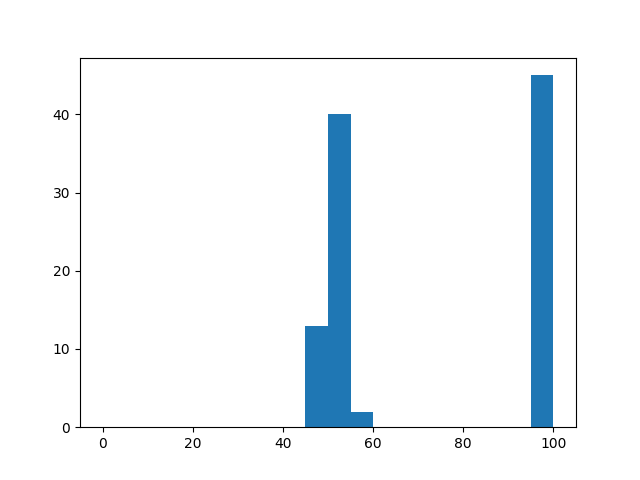
\includegraphics[width = 72mm]{figures/histograms/factor1/manual/5-01}
\caption{$d = 5, \lambda = 0.01$}
\end{subfigure}
\begin{subfigure}{7cm}
\centering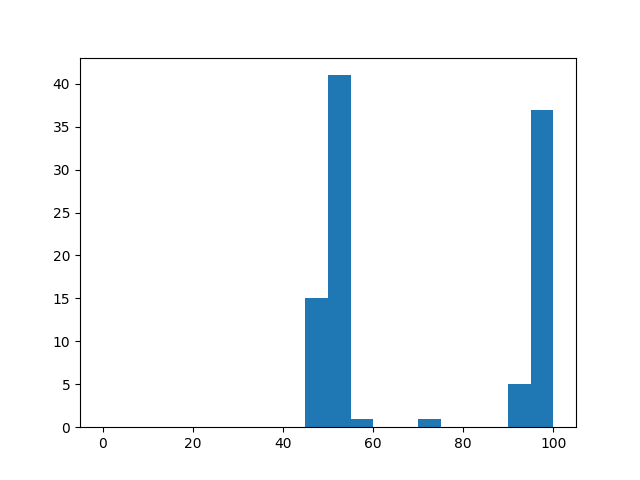
\includegraphics[width = 72mm]{figures/histograms/factor1/manual/5-001}
\caption{$d = 5, \lambda = 0.001$}
\end{subfigure}
\begin{subfigure}{7cm}
\centering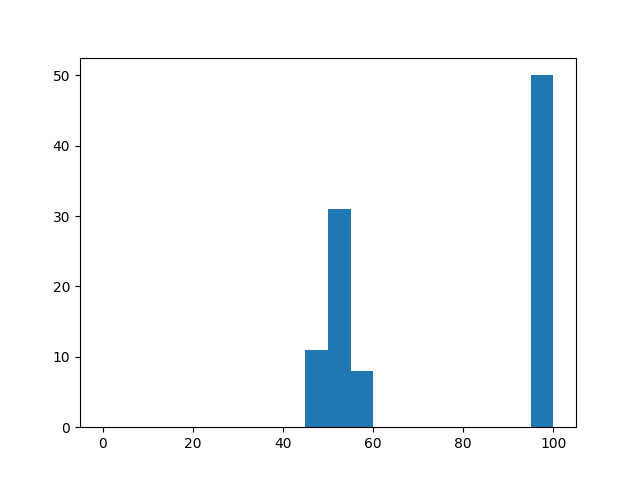
\includegraphics[width = 72mm]{figures/histograms/factor1/manual/10-01}
\caption{$d = 10, \lambda = 0.01$}
\end{subfigure}
\begin{subfigure}{7cm}
\centering\includegraphics[width = 72mm]{figures/histograms/factor1/manual/10-001}
\caption{$d = 10, \lambda = 0.001$}
\end{subfigure}
\begin{subfigure}{7cm}
\centering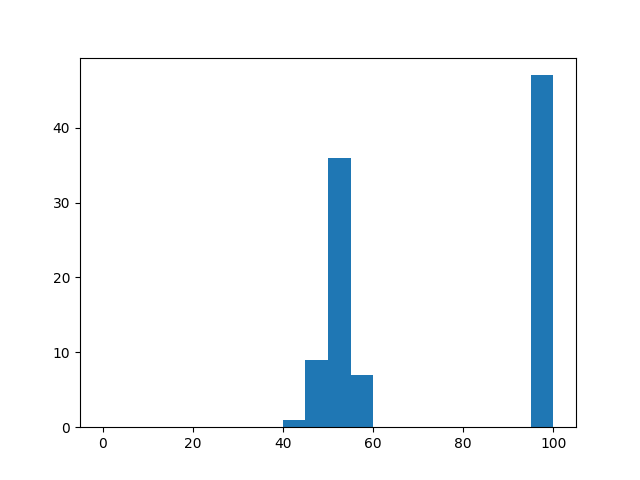
\includegraphics[width = 72mm]{figures/histograms/factor1/manual/20-01}
\caption{$d = 20, \lambda = 0.01$}
\end{subfigure}
\begin{subfigure}{7cm}
\centering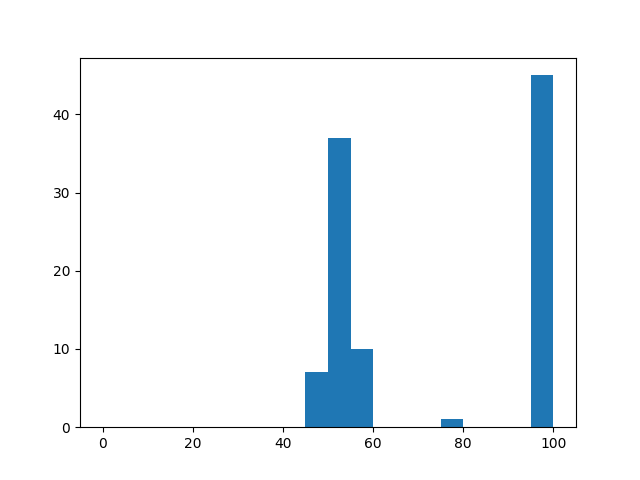
\includegraphics[width = 72mm]{figures/histograms/factor1/manual/20-001}
\caption{$d = 20, \lambda = 0.001$}
\end{subfigure}
\caption{Factor1}
\end{figure}

\begin{figure}[H]
\centering
\begin{subfigure}{7cm}
\centering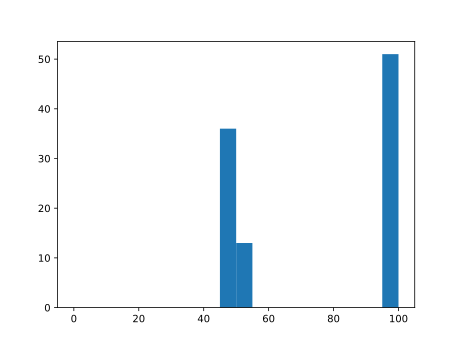
\includegraphics[width = 72mm]{figures/histograms/factor5/manual/5-01}
\caption{$d = 5, \lambda = 0.01$}
\end{subfigure}
\begin{subfigure}{7cm}
\centering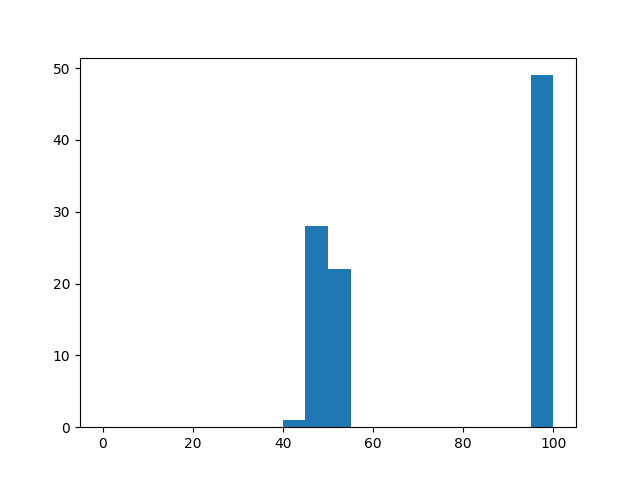
\includegraphics[width = 72mm]{figures/histograms/factor5/manual/5-001}
\caption{$d = 5, \lambda = 0.001$}
\end{subfigure}
\begin{subfigure}{7cm}
\centering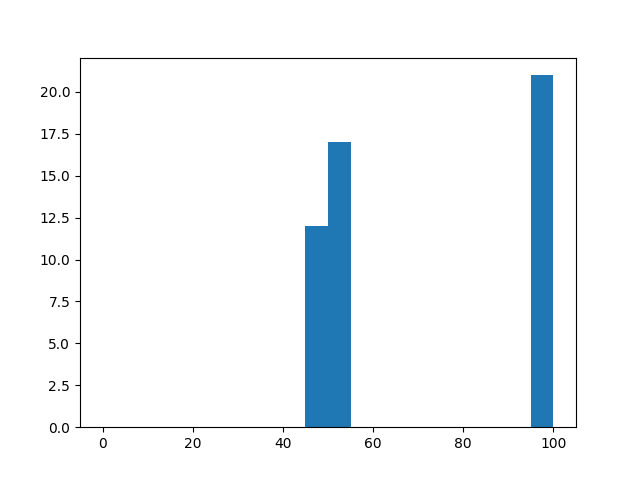
\includegraphics[width = 72mm]{figures/histograms/factor5/manual/10-01}
\caption{$d = 10, \lambda = 0.01$}
\end{subfigure}
\begin{subfigure}{7cm}
\centering\includegraphics[width = 72mm]{figures/histograms/factor5/manual/10-001}
\caption{$d = 10, \lambda = 0.001$}
\end{subfigure}
\begin{subfigure}{7cm}
\centering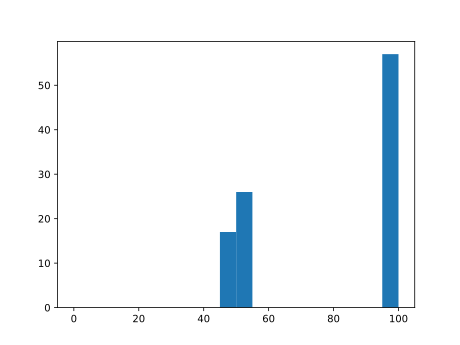
\includegraphics[width = 72mm]{figures/histograms/factor5/manual/20-01}
\caption{$d = 20, \lambda = 0.01$}
\end{subfigure}
\begin{subfigure}{7cm}
\centering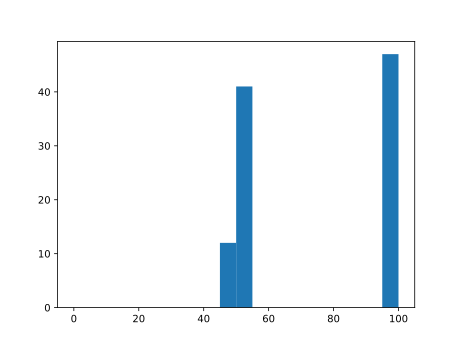
\includegraphics[width = 72mm]{figures/histograms/factor5/manual/20-001}
\caption{$d = 20, \lambda = 0.001$}
\end{subfigure}
\caption{Factor5}
\end{figure}

\subsection{Passing Representations to LSTM}

Now we pass the whole language representation ...

%\begin{figure}[H]
%\centering
%\begin{subfigure}{7cm}
%\centering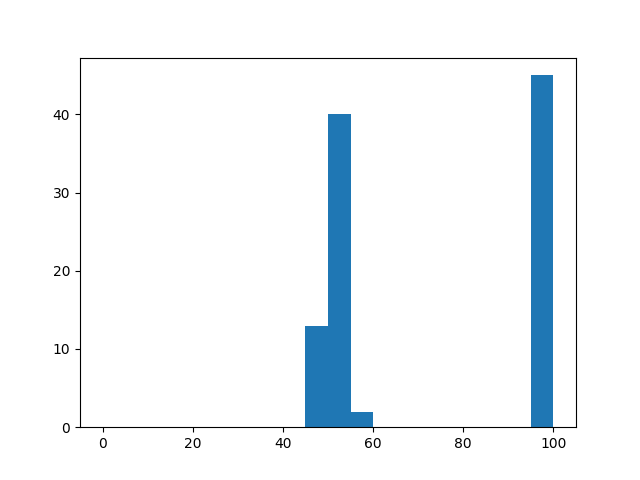
\includegraphics[width = 72mm]{figures/histograms/factor1/manual/5-01}
%\caption{$d = 5, \lambda = 0.01$}
%\end{subfigure}
%\begin{subfigure}{7cm}
%\centering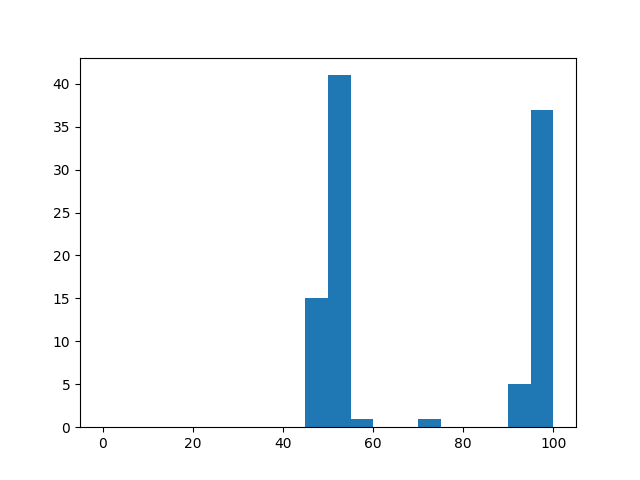
\includegraphics[width = 72mm]{figures/histograms/factor1/manual/5-001}
%\caption{$d = 5, \lambda = 0.001$}
%\end{subfigure}
%\begin{subfigure}{7cm}
%\centering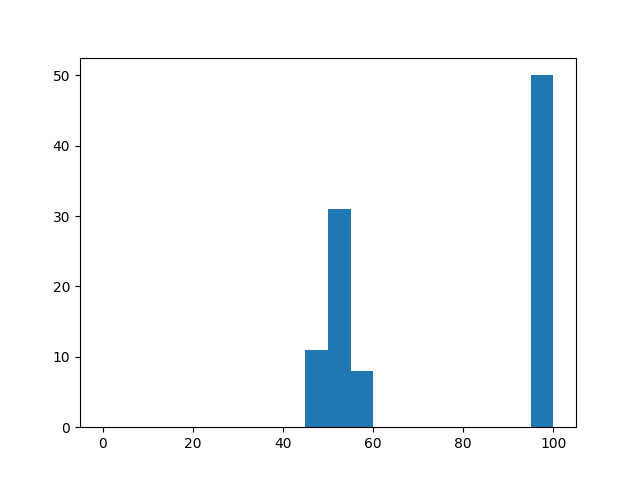
\includegraphics[width = 72mm]{figures/histograms/factor1/manual/10-01}
%\caption{$d = 10, \lambda = 0.01$}
%\end{subfigure}
%\begin{subfigure}{7cm}
%\centering\includegraphics[width = 72mm]{figures/histograms/factor1/manual/10-001}
%\caption{$d = 10, \lambda = 0.001$}
%\end{subfigure}
%\begin{subfigure}{7cm}
%\centering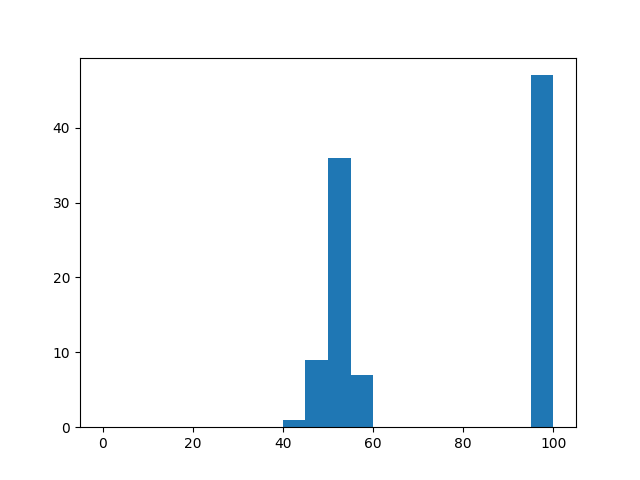
\includegraphics[width = 72mm]{figures/histograms/factor1/manual/20-01}
%\caption{$d = 20, \lambda = 0.01$}
%\end{subfigure}
%\begin{subfigure}{7cm}
%\centering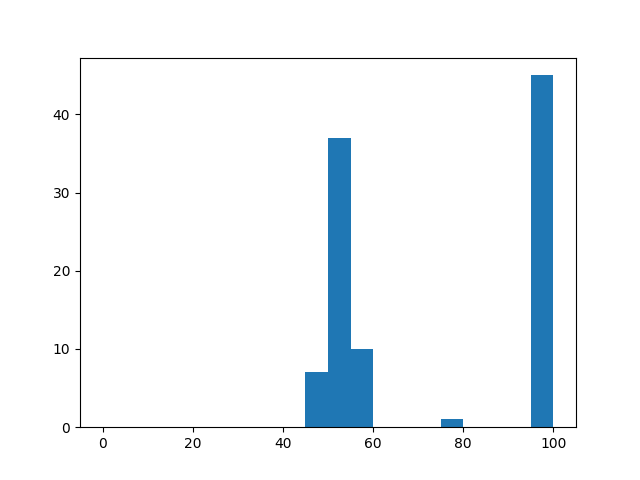
\includegraphics[width = 72mm]{figures/histograms/factor1/manual/20-001}
%\caption{$d = 20, \lambda = 0.001$}
%\end{subfigure}
%\caption{Factor1}
%\end{figure}

%\begin{figure}[H]
%\centering
%\begin{subfigure}{7cm}
%\centering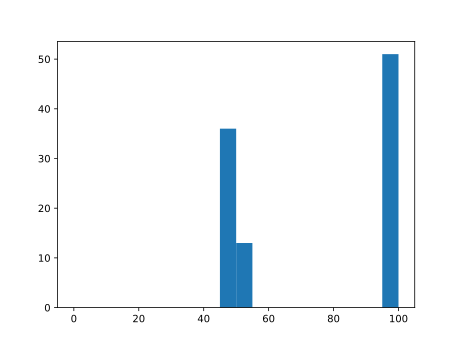
\includegraphics[width = 72mm]{figures/histograms/factor5/manual/5-01}
%\caption{$d = 5, \lambda = 0.01$}
%\end{subfigure}
%\begin{subfigure}{7cm}
%\centering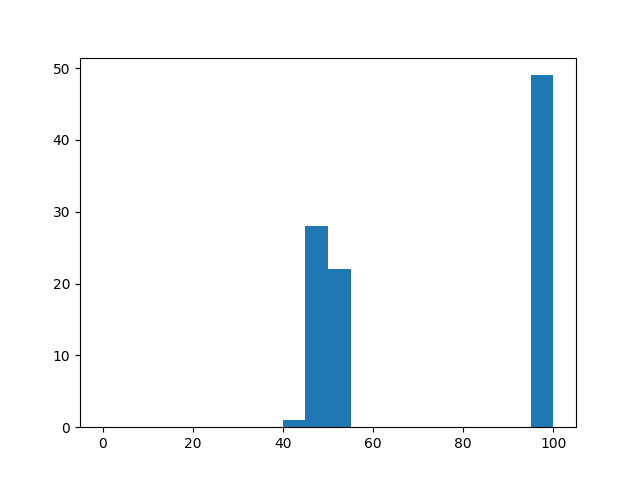
\includegraphics[width = 72mm]{figures/histograms/factor5/manual/5-001}
%\caption{$d = 5, \lambda = 0.001$}
%\end{subfigure}
%\begin{subfigure}{7cm}
%\centering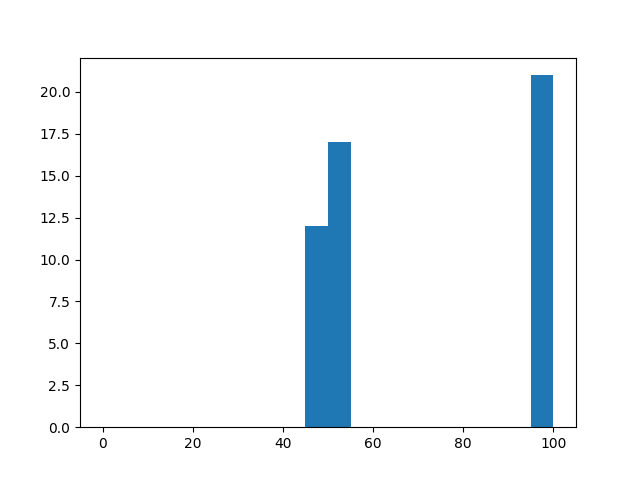
\includegraphics[width = 72mm]{figures/histograms/factor5/manual/10-01}
%\caption{$d = 10, \lambda = 0.01$}
%\end{subfigure}
%\begin{subfigure}{7cm}
%\centering\includegraphics[width = 72mm]{figures/histograms/factor5/manual/10-001}
%\caption{$d = 10, \lambda = 0.001$}
%\end{subfigure}
%\begin{subfigure}{7cm}
%\centering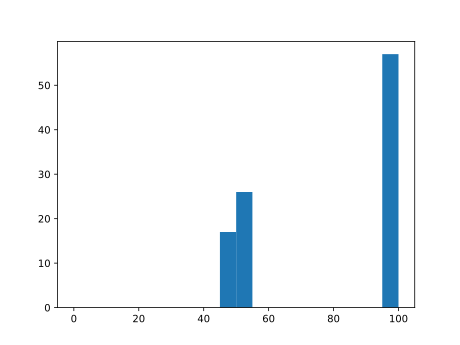
\includegraphics[width = 72mm]{figures/histograms/factor5/manual/20-01}
%\caption{$d = 20, \lambda = 0.01$}
%\end{subfigure}
%\begin{subfigure}{7cm}
%\centering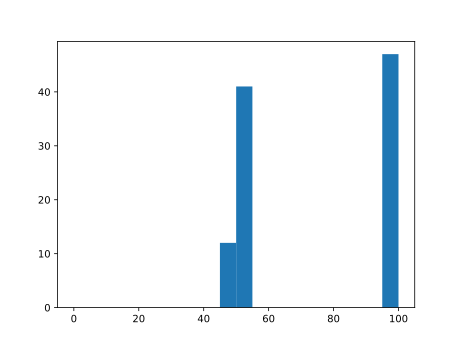
\includegraphics[width = 72mm]{figures/histograms/factor5/manual/20-001}
%\caption{$d = 20, \lambda = 0.001$}
%\end{subfigure}
%\caption{Factor5}
%\end{figure}

\subsection{Using Positional Encodings}

One of the problems of ...

\subsection{Supervising LSTM Gates}

\chapter{Discussion and Future Work}

\normalem
\printbibliography

\end{document}